\section{Sprint 2 conclusion}\label{sec:sprint2-conclusion}
This section concludes the preceding chapter on sprint 2.
It will conclude what knowledge was gained based on the sections of the chapter, and discuss a retrospective of the sprint as a whole, and what changes were made to the progress for upcoming sprints.

\section{Current product}
To give an overview of the progression of the project this section will provide an overview of what has been created during the sprint.
This overview will be split into two categories, to reflect the structure of the project: Networking and game.

\subsection{Networking}
The network aspect has been a big focus this sprint and has led to a better understanding of how the data should flow through the system (\autoref{sec:sprint2-deploymentdia}), and how the knowledge from sprint 1 about networking can be used to automatically find on-going games on the local network (\autoref{sec:accessonnetwork}).

From an implementation perspective, this sprint has introduced an initial version of the UDP host which is capable of transmitting Pozyx location data from the host computer to the game clients.
For the host, an initial console-based setup has been created, where the user can input the number of players, the location of the anchors as well as specify which tags are used in the game.
Additionally, the host can automatically re-order the list of entered anchors to ensure that they are sent to the clients in a clockwise manner, such that Unity can create a playing field mesh based on the coordinates.

\subsection{Game}
For the game aspect of the project, the most crucial parts have been implemented this sprint:\\
First of all, the game has been set up to support VR glasses by splitting the game view into two halves, one for each eye, as seen on \autoref{fig:initialvr}.

\begin{figure}[H]
	\centering
	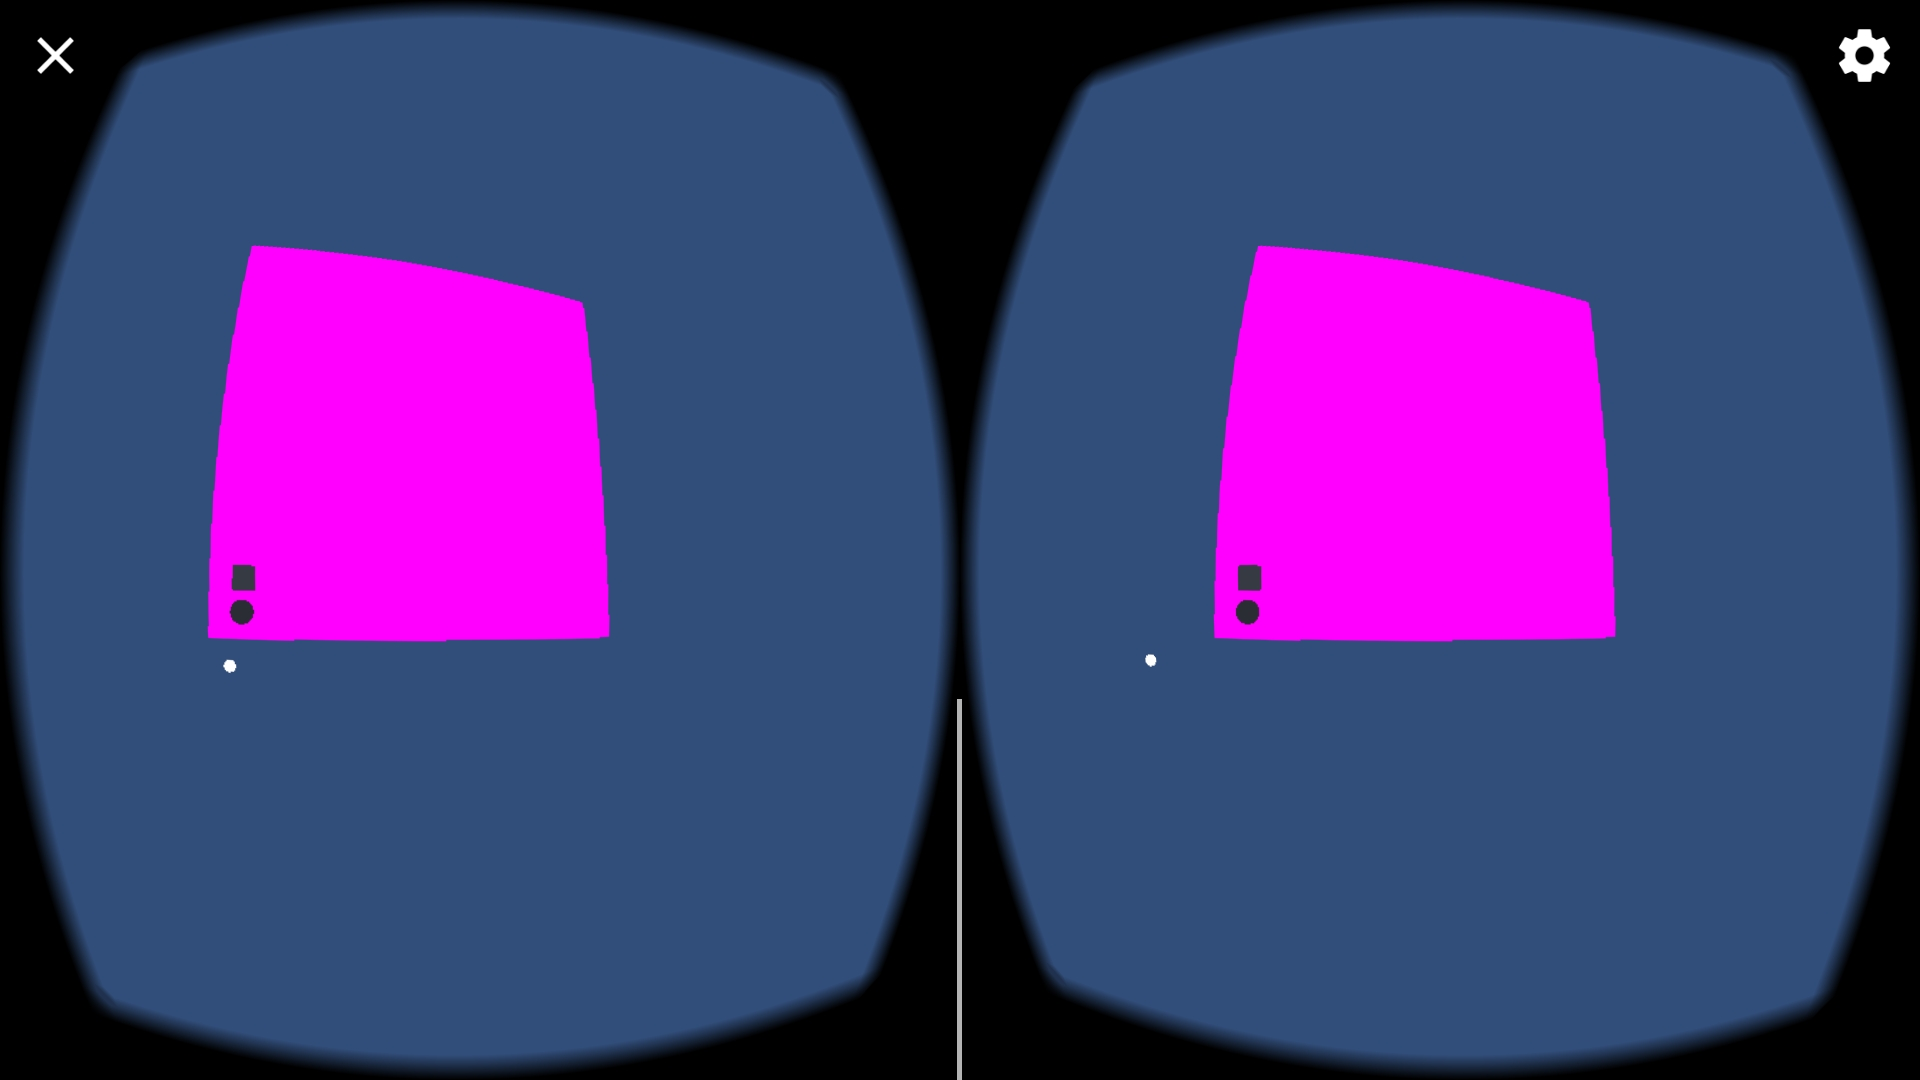
\includegraphics[width=0.6\linewidth]{sprint2/initialvr.jpg}
	\caption{The first implementation of VR}
	\label{fig:initialvr}
\end{figure}
\noindent
The game supports moving the players upon receiving new information from the host, but the connection between the two was not coupled together in this sprint.
Finally, an algorithm was implemented to generate the goal zones and ensure that they are placed fairly on the playing field.


\subsection{Retrospective on the process}
The process required some unexpected pivots in the second sprint due to the corona virus, which lead to the university being locked down for a period.
\\
The daily group work was moved from the physical group room to a virtual setting facilitated by Discord.
One of the major differences was that it was previously possible to sit down and do the pair reviews in the morning, which meant that reviews could be completed quickly and easily.
While we tried to still get the pair reviews done first thing in the morning, there was a noticeable delay before the new features were reviewed and merged.
Another minor change was how we assigned points (cost, reward, priority) to tasks. This worked out fine online, as people could simultaneously post their chosen number in a chat, as opposed to showing a number of fingers while sitting around a table.
\\\\
Since most of the project work is managed on Jira and completed by individual group members, there was not a noticeable change in the amount of work getting done.
A side effect of working with only voice chat was occasional difficulty in reaching the other members when their help was needed since they might be temporarily away from the computer, or too distracted or focused to be paying attention to the voice chat.
This also resulted in some information not getting spread to the entire group, as not everyone may have been listening while a discussion was happening, which led to minor confusion in further discussions on the subject.\\\\
Like at the end of sprint 1 (\autoref{sec:sprint1-conclusion}), a retrospective was conducted by the anchor to reflect upon how the process was working out.
In addition to discussing the progress of the project, the following points were brought up:

\subsubsection{How does the process with Jira work?}
Currently, it seems like the challenger is the only person adding suggestions to the backlog.
After some discussion it turned out that multiple members thought that this was intentional, and did not know that they were also supposed to contribute with their suggestions for the project.
This has been clarified, and all members are now aware that they are fully encouraged to add suggestions to the Jira when they come up with ideas for the project.

\subsubsection{Should we use pair programming more?}
Right now, the only work done in pairs is the pair reviews.
It was decided that utilizing pair programming for larger programming tasks would be beneficial to attempt to decrease the amount of time spent on it and allow for more perspectives on implementation.
Whether or not a task should be done with pair programming will be decided as a part of the task discussions that take place after the daily stand-ups if there are new tasks in the suggested column.

\subsubsection{How do we give better estimates about when a task is done in daily stand-ups?}
Generally, the biggest reason that it is difficult to estimate how much remains of a given task, is that the definitions of done are not precise enough.
To combat this, it was decided to remove the prioritization of tasks where we would assign a reward, cost, and priority.
Instead, the discussion will be about what a good and specific DoD is for the given task to ensure that everyone is on the same page.
The hope with this approach is that discussing the DoD will give new perspectives to a given task, and shift the focus from how long it will take to complete the task to exactly what needs to be done.
A possible by-product of this shift of focus is that the in-depth discussion will result in discovering new tasks that need to be completed.

\subsubsection{How do we feel about daily stand-ups?}
Everyone is generally pleased with the daily stand-ups, but there is a tendency to focus more on what has already been done rather than what is currently being worked on.
To prevent this, a new format for the meetings has been proposed:

\begin{itemize}
	\item{What have I been doing? (short answer)}
	\item{What am I working on now?}
	\item{When will my task be completed?}
	\item{What is my current challenge?}
	\item{Do I need help or reviewers?}
\end{itemize}
\noindent
After each member has presented these five points, we will go through the new tasks in the suggested column and define a DoD for them.
Finally, we went through all tasks that had been completed in the sprint to ensure that everything that had been implemented was also documented in the report, to ensure that the knowledge is shared between all members of the group.
